\part{SOA}


\chapter{Overview}



PHP本身只是一个单线程的Web开发及系统集成的脚本开发语言。


并发请求是指将一组多个API调用的名称和参数分发给多个服务器同时执行待所有api都执行成功并返回结果后将结果整理一起返回给请求方,​当然也可以使用线程来完成,但是PHP的单线程特性不适合处理并发请求,需要使用Swoole扩展来和其他服务器进行通信。

​当请求一个接口时,执行完毕后需要把结果返回给调用者后才能继续执行下一跳指令的请求就是同步的,异步请求只要把请求下发,不需要等待返回结果就可以执行下一个操作的请求是异步的,不会阻塞代码执行,不过也可能在某个时刻聚合执行结果。

PHP处理每个请求时都需要重新加载并解析一次脚本,平时流量不多的时候看不出来,当业务发展后业务复杂度增加而PHP加载的文件越来越多,磁盘IO负载不断增加,并发请求增多导致磁盘效率下降,最终每次请求都会渐渐变慢。为了解决这个问题,可以使用opcache扩展缓存PHP解析后的代码,文件如果没有更新则只需解析一次后就一直在内存中。

PHP从持久层获取来的数据也不会有任何内存保存(当然其他常驻内存的语言即使能做到但也不会这么做,因为会因为数据不同步导致脏数据)当流量不断增加的时候持久层一直是个单点服务器(主从后主库也是唯一单点)前端服务器可以横向扩展但是单点的持久层是不能增加的,最后导致大量的持久层拆分及相关繁琐事宜。为了解决这个问题,可以使用Memcache或Redis缓存热数据或启用其他分布式事务持久层。如果没有统一的方案,只能使用架构针对业务特有环境特性适配各种缓存方案(例如分库分表)。

PHP不是常驻内存,导致很多特殊服务无法实现,必须依赖外部服务。例如,计数服务只能依靠C或Redis等服务实现,而且PHP本身的扩展对于通讯及进程类支持很弱,因此无法使用PHP开发分布式计算和数据挖掘等,不过现在PHP7.0开始支持强类型,而且可以使用Swoole等强化网络通信功能。

PHP没有强制的框架规范,无法统一制定开发标准和划分模块及项目,例如在通过Socket请求RPC服务等操作时只能采用一个隔离性极强的方式去实现。

PHP的单进程单线程模式在当处理复杂的业务的时候只能串行执行命令,所以CPU、磁盘、内存等的利用率都很低,很多任务都需要排队等待,需要使用pthead等扩展才能并发地执行多任务以及返回结果。或者,可以通过隔离前后端的方式来处理复杂业务,前端可以通过消息中间件,同步或异步地调用一个或多个接口,但是PHP的socket扩展使用成本很高。

PHP无法解决资源争抢问题,当使用持久层时往往有些关键数据是不能及时同步的,例如库存剩余和抢购等高并发业务都需要在持久层或者前端进行大量的拦截和锁定,但是实际情况是持久层压力很大的同时,很多其他无关的业务也受到影响。虽然可以使用队列,但是PHP支持的队列并不多,而且对全局单个数据或事务锁定的支持不完善,往往只能直接在持久层锁定或使用Redis,Java可以使用zookeeper等实现分布式支持来解决高并发问题。

PHP不能很好的解决单个文件并发写的问题​​,当业务产生错误时无法及时的预警,文件无法异步写只能等待写完后才能解除锁定,虽然可以使用扩展插件来尝试解决并发写问题,并且将分布式日志集中监控管理来处理异步写操作,不过大部分语言都无法很好地解决这个问题。

PHP无法解决文件共享问题,可以和PHP配合使用的分布式文件存储系统很少,往往只能先写到Redis,再使用异步队列进行处理。

PHP无法处理并发流量增加后的资源争抢严重的问题,MySQL主从延迟往往会超过30秒,这样当PHP查询一个用户是否点过赞时,从库需要很长时间才能同步,这种情况下需要在前端使用cookie加锁,并对服务加上公共锁(setnx+expire),还可能要使用悲观锁和乐观锁。

PHP的缓存解决方案往往只能使用Memcached等,但是使用Memcached来存储很多无用数据时会导致Memcached不断地在不同大小的slab中存储数据,这种情况需要多个Memcached集群并且规划数据缓冲规则,Memcached无法缓存超过1M的数据。

PHP无法解决Memcached脏数据问题,需要集中封装底层DAO,一旦数据发生变更就自动更新相关cache,如果更新频率极高则需要使用Redis进行存储,同时还需要​确认前端哪些部分的数据是需要设置过期时间等。


PHP框架中模块层级太多就会导致代码很难被重复调用,而且模块划分不清晰还会造成很多数据重复获取,需要引入依赖注入或类自己本身缓存一些数据,但是也可能是过时的数据,还可能导致PHP内存溢出。

PHP无法常驻内存以及对数据持久层依赖太大等问题,需要考虑使用MySQL代理以及Redis一致性Hash代理等尝试解决。

PHP不支持长连接以及异步并发调用的问题可以考虑使用Swoole、Socket、Libuv和Libevent等尝试解决。

在实际的应用中用到的Swoole的特性包括TCP定长包头非定长body通讯协议,客户端长连接,task同步异步处理业务逻辑并定期重启(清理未回收资源),worker接收task结果并判断是否全执行完毕以此返回结果(并发处理任务),客户端超时以及worker进程管理。​













\chapter{Dora-RPC}

随着业务和规模的扩大,需要对很多服务和操作进行抽象和隔离,通过分层操作把服务划分为前端服务和后端服务,并且尝试通过隔离项目来管理各个项目之间的依赖关系。例如,业务层可以划分为订单服务、用户中心、权限管理和查询服务等,底层服务可以划分为分词服务、队列服务、推送服务、计数服务、短信服务和邮件通知服务等。

拆分带来的好处就是可以向平台化更进一步,其中前端承载展示界面并拼装组合来调用后端的业务和服务,后端业务逻辑不承压,但是需要处理各种复杂的业务逻辑,而且后端本身是一组或多组独立的简洁的业务逻辑封装模块,它们为前端提供了丰富的标准化的接口。

上述的架构演进其实是逐渐向SOA发展,而且SOA在抽象良好的情况下可以集成不同的功能。例如,使用前端的逻辑快速的将过去的服务接口拼装出各种所需业务或者一个业务执行了对外订阅的业务发送通报,怎么处理只需要其他业务根据需要来决定。

项目越复杂隔离性越重要,因此SOA实施的过程中需要架构和开发人员不断抽象总结,最终组织出标准化的后端的接口,而且SOA需要有很多底层服务的支撑才能完成。

有很多场景并不适合使用SOA来实现,例如内容发布系统只要生成静态页面,那么使用接口就可以满足,不断变化迭代的项目反而不适合使用接口。

SOA中的依赖管理可能会很复杂,所以需要对需要对外公开的服务进行规划,并分析好现状以明确哪些项目适合,哪些不适合,因此Java有自己的集成消息总线及中间件和标准等。

相比SOA,RESTful并不适合互联网,只是简单的增删改查并不能诠释API的所有功能,RESTful适合封装数据接口,但是业务接口事实上是SOA里面最重要的组成部分之一。


Dora RPC 是一款基础于Swoole定长包头通讯协议的最精简的RPC,可以用于复杂项目前后端分离,分离后项目都通过API工作,可以更好的跟踪、升级、维护及管理。

Dora-RPC旨在使用PHP来实现一个企业级的SOA业务架构,通过这个架构可以快速实现如下的功能:

\begin{compactitem}
\item 内部SAAS及完善的监控管理
\item 动态可伸缩式的后端
\item 更简单的内部API集成管理
\item 分布式调试支撑
\end{compactitem}

在使用SOA来分离前后端后,用户的一个请求过来后前端往往会产生平均10到200个请求到后端以完成一个用户​一次的页面请求,因此常规的数据请求接口和业务接口需要有明确的划分,否则页面渲染会很慢还难以降低后端压力,实际运行的效率也很低,因为这些接口很有可能是串行调用,并且是逐个阻塞执行的。

业务接口权限往往权限很大,而且端口回收速度很慢,因此除了让前端直接和后端通信之外,还可以使用中间件对消息进行转发和控制,这样就可以通过检测应用服务器的返回结果来判断后端服务器是否太忙或者宕机,从而通过PHP代码将故障机摘除或者降低投放任务量,并将失败的请求转发到其他存活的应用服务器。


\section{Overview}

Dora-RPC使用Swoole扩展进行再次封装来实现PHP的前后端分离,当项目变得庞大的时候需要隔离一些功能作为公共服务,Dora-RPC希望可以将复杂的系统通过API服务变的简单和易维护,同时更好评估复杂项目和跨项目组调用更加清晰。

前后端分离的好处是可以减少业务抽象接口的代码依赖,并且根据日志记录统计调用频率分布,与此同时带来的不足就是通信压力增大,需要使用Swoole等作为PHP的RPC通信支撑。

如果一个用户请求的前端过多仍旧会很慢,需要对展示结果没有影响的处理发送到后端异步执行,执行没有先后顺序的请求并发下发到后端应用服务器并发执行等都有结果后一起返回结果,但是这也导致了持久层会承受很大压力,每个请求过来后都会并发下发10到20个并发任务给后端去处理。

如果前端发送4000个请求,后端就要并发80000个处理进程,而且还是瞬时并行的,要求后端数据服务连接数也同时增加20倍。例如,在使用Swoole实现PHP连接池时需要启动大量的worker进程,往往一个服务器就至少启动了4000个task。









\begin{figure}[htbp]
\centering
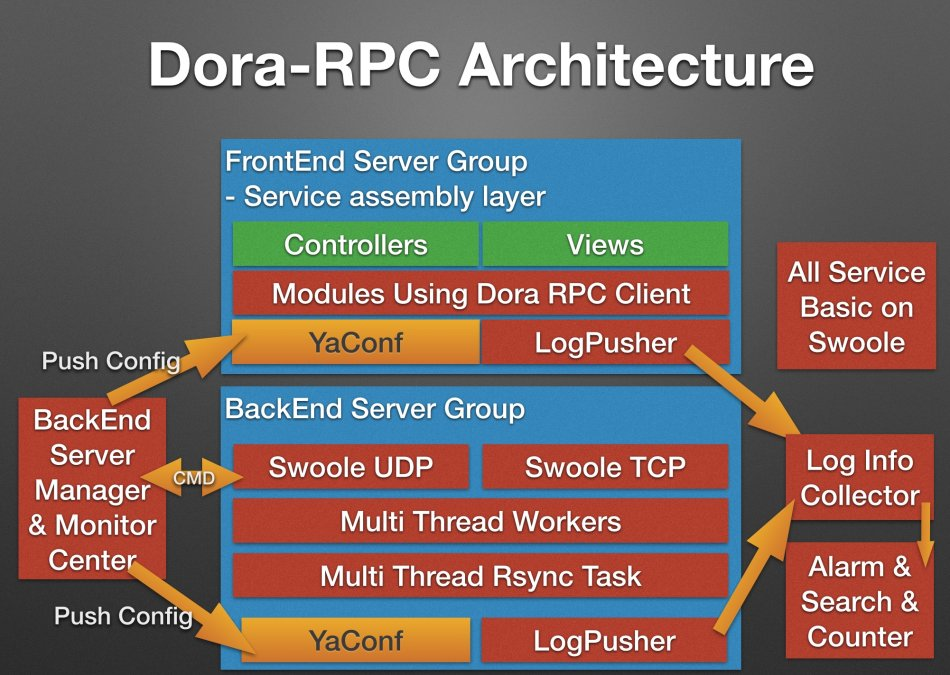
\includegraphics[scale=0.3]{dora-architecture.jpg}
\caption{Dora-RPC架构}
\end{figure}

Dora-RPC将服务器分为两组:前端和后端,其中前端负责展现和拼装,复杂的业务逻辑由后端负责处理。

\begin{compactitem}
\item 前端:负责承载服务请求,对后端提供的服务进行拼装。支持同步、异步、单个、多个 任务下发。
\item 后端:负责提供类似FPM的容器常驻内存接收前端请求。
\item 监视服务:负责监视后端工作状态及配置同步
\item 日志服务:日志收集及统计,服务预警及日志查询。
\end{compactitem}

目前Dora-RPC的实现只完成了基础的RPC功能,支持同步、异步、单个、多个任务下发,缺少的功能如下:

\begin{compactitem}
\item 本地日志监控及推送(swoole的process实现)
\item 分布式日志统计及收集
\item 分布式调试日志及查询
\item 日志查询及索引
\item 预警通知系统,支持邮件,短信,及自定义模块
\item 后端前端服务器监控及界面
\item 配置同步管理及推送机制
\item 更好的监控规则
\item 容器工作状态监控
\item 异步队列
\end{compactitem}

Dora-RPC框架仅提供一套最基本的服务端和客户端,通过简单集成即可使用在任何开发框架上。


Dora-RPC框架返回的数据结构分为三层,每层都有msg和code,第一层(底层)代表当前客户端通讯情况,第二层代表当前api在服务端执行情况是否有异常或者投递情况,第三层代表代码执行情况,例如如果业务代码产生异常自动会记录在这里,使用这个方式是因为RPC本身的复杂性,通过提供这个方式可以判断系统真正的状态。

Dora-RPC框架底层升级来支持异步任务,服务端处理完异步任务后会向客户端发送处理结果,如果当前客户端向服务端下发新任务并执行Recive的时候,之前客户端是无法判断出这次返回的内容是否为此次请求,与此同时由于长链接的特殊性,上一次的请求如果被异常中断没有执行recive的话,会导致上次的结果被本次请求拿到。为了防止以上问题,Dora-RPC使用guid判断完成了异步任务结果的收集和非本次请求的返回数据的鉴别。

生产环境中的复杂的业务代码不能保证不会因为一些特殊原因产生故障,而且很多故障会导致进程终止,为此业务代码都是在task上执行,而不是worker上,这样就可以实现很多特殊的功能。

Dora-RPC支持服务分组,很多情况下的服务是在一个公共池中,不可避免地都会受到影响,而且不同业务部署在不同的服务器上也很常见,这些都要求Dora-RPC可以提供服务分组功能,规定某个服务器属于哪几个组,通过组能找到正确的服务器配置进行连接工作。



在Dora-RPC的任务下发模式中,下发任务数量可以分为如下:

\begin{compactitem}
\item 并发多个任务下发
\item 单个任务下发
\end{compactitem}

下发任务等待结果有多个模式,例如:

\begin{compactitem}
\item 下发任务阻塞当前进程等待处理完毕并拿到返回数据
\item 下发异步任务不等待任务处理结果,只会返回下发成功,而任务在服务器跑完毕后没有任何返回
\item 下发异步任务不等待任务在服务器的处理,下发成功后马上返回下发成功,而服务完成后服务端返回处理结果给客户端,客户端通过一个函数统一将所有之前异步任务结果获取返回给当前业务进程。
\end{compactitem}

通过以上方式,Dora-RPC可以成倍的增加接口响应速度和服务器利用能力,即使不使用复杂的多线程也可以达到相同的目标。 

在Dora-RPC的网络通信中,客户端可以在PHP-FPM及CLI下工作,并且可以维持长链接。

每次来回一次请求网络耗时在 0.002~0.004 左右(也取决于内网网络),请求处理完毕后链接仍旧保留不关闭 减少握手耗时及客户端队服务器的端口数消耗。


RPC单线程客户端和虚拟机下的测试QPS大概在200~500次每秒通讯,每次下发的任务可以很多,在单应用服务器中的QPS可以达到2000。



\subsection{Gzip}


若数据较大,支持包压缩gzip若有特殊需要可简单更改为其他压缩方式。

\subsection{Serialize}


序列化使用的PHP自带的serialize,若有需要可以直接自行更换。

\subsection{Timeout}


连接和接收结果默认超时3秒,在const文件内设置,如果出现超时,客户端会自动使用其他配置进行尝试重试指定次数后返回json描述错误原因。如果有需要可以在重试逻辑内增加重试监控,监测各个服务器的工作状态。

\subsection{IPFilter}

如果在本次请求中有一个ip已经失败过一次会自动在本次内进行屏蔽,如果发现所有配置已经都尝试或超过重试次数会返回失败。cli下失败一次后再次下发API时会取消掉之前所有屏蔽配置继续重试。

\subsection{Proxy}

客户端连接反向代理会消耗一定时间,因此Dora-RPC当前的通讯架构并没有加入反向代理服务,而且反向代理服务器虽然性能高但是本身也是一个“单点”,对于分布式服务来说还是直连方式比较方便。





对于PHP开发者来说,很少使用PHP实现大型的复杂的软件,因为开始的时候就会下意识的将项目拆分成小的组件,然后通过各种各样的API相互调用,以此来避免过于庞大的代码维护和跨部门调用。


如果使用模板引擎,并且在项目快速迭代时很容易出现的情况就是代码的相互依赖越来越严重。例如,一个项目可能需要集成三个到五个以上的项目提供的服务,这种情况下如果在底层更改了一个字段的名称可能就会造成大量系统不能正常工作的情况,在执行这类修改时如果修改人没有充分的“觉悟”是不会通知其他开发人员的,而且这种事情在PHP环境下发生之后并不是马上就能发现的(系统往往会用不存在的字段作为判断条件而导致逻辑工作方向异常。

如果要实现在开发过程中主动发现这类问题,需要将一个复杂的问题简化到一个级别后才能进行管理,这需要一个过程和切入点将一团乱麻的项目进行切片。

现实中,业务集成前端和后端的复杂度是不同的,在服务化的情况下我们可以很快的利用原有的服务能力拼装出各种丰富多样的界面和服务,而且通过服务化恰好的能够将后端的分布式复杂性和并发性与前端业务的组合复杂度完全的隔离开。

最好的效果就是即使后端底层把一个数据库被替换了或宕机了,在接口上层也不会感受到有任何变化,服务依旧稳定完整运行。通过这个方式我们还可以对我们的服务进行管理——包括功能完善、性能测试、对接口变更及依赖进行监控等以此来提高对外服务的稳定性,也可以加强对内服务的把控。

后端的复杂性的原因其实是后端服务为了一致性造成的成本是十分昂贵的,而且这不仅仅是硬件的投入,还有大量的人力消耗。例如,在互联网初期建设的时候,后端的压力承受能力有限、设备及服务昂贵,为了提高MySQL的查询QPS就需要通过大量的主从横向纵向表拆分的工作,虽然可以人工用大量的技巧解决了这个问题,但是实际上消耗还是很庞大的,而且没有人能够完全脱离业务做出一个通用的公用的可随时根据流量扩展的数据服务。

在出现了很多分布式的数据处理服务之后,但是这并不意味着后端的数据和缓存是简单容易的,而且现代的后端仍然把大量的注意力集中在“业务实施”上,很少有开发者关注一些更底层的服务。


在实际生产环境中,100万PV和20亿PV的网站的区别是很大的,主要体现在服务化和自动化管理以及后端是分布式可扩展的。

在初级阶段,只是通过增加一些缓存来减轻后端数据服务压力,往往没有完善的服务治理,现实中的业务驱动则往往要求任何网站不仅仅要关注自己的业务实现,如果条件允许还要实现服务化、自动化和平台化。

事实上,服务化、自动化和平台化都是基础服务的基础支撑,只有具备了这些系统后才能提高内部的灵活性,反过来如果做的很糟糕或者很复杂,那么基础服务往往成为了累赘。

Java本身就是一个复杂工程化的语言,因此Java是最早提出消息中间件、微服务、分布式、一致性概念的,对于大流量、大数据、高并发处理提供了大量开源实现,因此分布式后端服务对于Java来说不是很新鲜的东西。

如果仅仅关注使用PHP实现业务,那么在更大流量的情况下往往就需要重新调整架构或者向其他架构迁移,业务本身就已经很复杂了,很难整理和完善底层了。

如果在PHP框架中充斥着语法糖等过渡方案,那么对于性能的优化和企业级别的架构支撑就不可能太理想,最起码没有提供很多分布式及服务化的基础服务,不过Zend、Symfony2、Laravel等已经开始向这个方向开始努力,开发者也开始关注如何大流量网站的底层实现。



服务化对于大型业务流量大的互联网公司帮助很大,从最初的隔离开前后端的复杂度,让业务的实现尽量不受后端的限制以及让变更更可控等,同时这些都已经在Java领域的服务治理思想上有所体现。

实际上,在把业务和数据抽象成服务之后只是让业务有了一定隔离,接下来还有更多事情需要实现。例如,现实中的服务器的本地端口只有65535个(实际可用的还要减少1000个),客户端短链接每次都需要重新握手链接,然后用完后要等待超时才能回收这个端口,并发高的时候端口会不够用,虽然转换成长链接可以缓解端口限制,但是如果前端进程数超过了后端服务器的可用端口数还是会出现这类问题。

前端接口在被用户调用后往往会访问后端服务很多次,例如100万PV的前端请求传递到后端可能是1000万次请求,对于这类请求放大会导致后端服务器必须要比前端服务多很多,如果服务器不多就仍然不能做这类事情。

所有服务都做成API对外服务也并不一定可以解决上述问题,如果访问特别频繁的话,除了通过一些精简和合并(例如数据服务一次取一条改为一次取多条来减少请求次数),需要拓展的视野不仅仅在HTTP协议。

虽然业务开发中出现了线程模型、进程模型和协程模型等不同模型,但是如果只是写业务逻辑,还是使用单线程的方式实现是最好管理和调试的。

虽然实际上单线程+单进程的实现方便维护和调试,但是导致的问题就是很多可以并发的任务变成串行化了,如果使用大量的多线程来实现前端业务,对于常规的开发方式来说是一场灾难,当然可以更好的优化方式(例如Nodejs方式的evenloop),不过这些方式虽然提高了CPU利用率,但是代价就是代码的维护成本比原先要高很多,后来才出现了Go的协程、PHP的Yield、Swoole的IO协程等方案。


单线程慢主要原因就是串行化执行代码到IO这些操作时阻塞导致了CPU空闲,Swoole的协程细化到所有IO操作可以让实际开发的时候无感,虽然Swoole的方式是最简单的无关注的,但是只能使用它规定的驱动,PHP的协程Yield实现了多个独立的代码块在人工发现有IO等待时调用它然后去处理其他的任务,虽然这可以实现一些灵活的调度,但不是所有人都能掌握,而且实现思路有些复杂。

在Go的实现中,多个并发任务的执行中分出来的“线程”有阻塞的话仍旧会阻塞等待,NodeJS使用回调实现了完全异步操作,但是代码复杂度的提升导致调试困难。

通过以上的分析对比后发现,最好是单线程写业务、并发任务能很简单的执行而无需关注底层协层细节是对于我们来说更好的实现业务的方式。


\section{Performance}

基于Vagrent分配1G内存和1核CPU来对Dora-RPC进行压力测试的配置和结果如下:

\begin{compactitem}
\item 压测进程:使用10个php进程发送请求
\item 并发性能:TPS 2100左右(比直接使用curl快很多)
\item 响应时间:0.02~0.04s
\item 后端代码为:查询一次数据库后返回结果
\item CPU使用:10\%~25\%
\item 内存使用:一个PHP task占用16M内存
\item PHP版本:5.4.41
\item 压测时使用端口个数:10个(长连接)
\end{compactitem}

测试代码使用的客户端示范程序无限循环,服务端直接返回一个数组,每次接口会请求一次api接口调用后再下发一个请求,其中内含两个并发任务。

\begin{figure}[htbp]
\centering
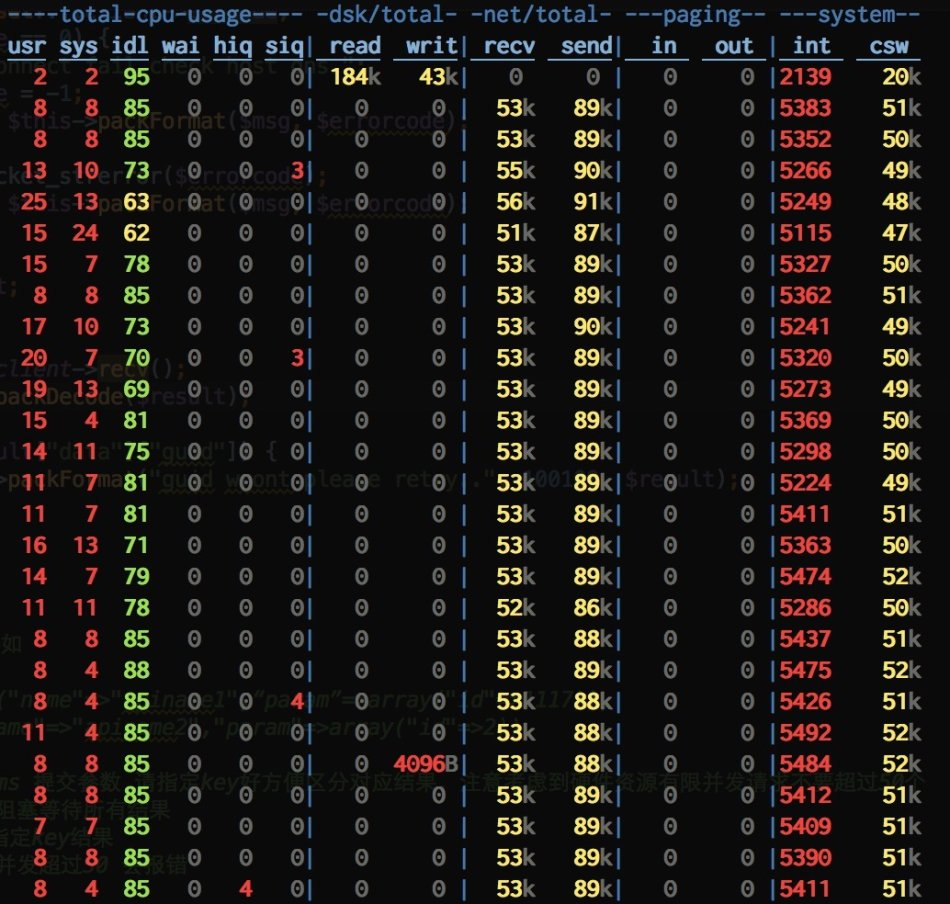
\includegraphics[scale=0.3]{dora-press-test.jpg}
\caption{Dora-RPC压力测试}
\end{figure}

\begin{compactitem}
\item 客户端使用长链接,处理请求结束后连接也不会断开,再次使用的时候会自动找回
\item 服务端自动管理task及进程通讯
\item 通过task处理业务
\item 如果使用更高速的序列化函数取代serialize会更快一些
\item 支持单api请求,多api并发请求,此功能可取代发展越来越怪的gearman
\item 如果有持久化请求需求,可以考虑在此基础上自行封装下(可能导致性能下降)
\end{compactitem}

另外,还可以增加中间件来检测后端服务压力状态和自动负载均衡。


\section{Service Discovery}


当服务器需要增加减少的时候,正常的流程是更新客户端的配置来实现新服务器的增加,但是这个方式有很多缺点。例如,如果某台服务器出现故障,短期内可能无法发现,发现后还是需要人工修改配置或去运维配置中心区进行摘除,通过服务发现则可以自动摘除。

增加服务器时,只要控制逻辑完善,后期可以让服务发现来把这个过程完全自动化。


Dora-RPC提供了最简单的服务发现实现方式,使用redis作为存储,记录所有服务端的ip和端口及所在分组。


启动应用服务器时,需要通知服务发现的redis列表,服务器会自动将当前服务的ip和端口及分组上报到多个redis上进行注册,并定期刷新其超时时间。如果有个别节点在超过超时时间仍旧没有再上报,那么自动摘除。


客户端会定期从多个redis获取到最新的配置,并且更新本地配置文件内容。

\section{Service Downgrade}


当服务器压力剧增的情况下,根据当前业务情况及流量对一些服务和页面有策略的降级,以此释放服务器资源以保证核心任务的正常运行。


服务降级方式包括服务接口拒绝服务、页面拒绝服务、延迟持久化以及随机拒绝服务等。

\begin{compactitem}
\item 服务接口拒绝服务:无用户特定信息,页面能访问,但是添加删除提示服务器繁忙。页面内容也可在Varnish或CDN内获取。
\item  页面拒绝服务:页面提示由于服务繁忙此服务暂停。跳转到varnish或nginx的一个静态页面。
\item 延迟持久化:页面访问照常,但是涉及记录变更,会提示稍晚能看到结果,将数据记录到异步队列或log,服务恢复后执行。
\item 随机拒绝服务:服务接口随机拒绝服务,让用户重试。
\end{compactitem}



\begin{longtable}{|m{50pt}|m{200pt}|m{150pt}|}
%head
\multicolumn{3}{r}{}
\tabularnewline\hline
数据操作动作&通过Cache工作&通过异步数据队列
\endhead
%endhead

%firsthead
\caption{服务降级 - 持久层降级方式}\\
\hline
数据操作动作&通过Cache工作&通过异步数据队列
\endfirsthead
%endfirsthead

%foot
\multicolumn{3}{r}{}
\endfoot
%endfoot

%lastfoot
\endlastfoot
%endlastfoot
\hline
增insert&禁止&允许但不能有重复问题\\
\hline
删delete&禁止&允许但不能有复合操作\\
\hline
改update&禁止&允许只留最后结果\\
\hline
查query&允许,若未命中问询mysql或其他持久层&走cache\\
\hline
\end{longtable}

降级方式可以包括直觉管理方式和分级管理方式,其中前者要求运维人员可以指定哪些模块降级,而后者则无需运维人员关心业务细节,直接按级别降低即可。


在直觉管理方式中,当服务器检测到压力增大时,服务器监测自动发送通知给运维人员,运维人员根据自己或相关人员判断后通过配置平台设置当前运行等级来降级。

降级首先可以对非核心业务进行接口降级。如果效果不显著,开始对一些页面进行降级,以此保证核心功能的正常运行。

在分级管理方式中,当服务器检测到压力增大时,服务检测自动发送通知给运维人员,运维人员根据情况选择运行等级从1到10,各个应用根据自己的级别自动判断是否工作和如何拒绝。


服务降级埋点的地方包括消息中间件、前端页面和底层数据驱动。

\begin{compactitem}
\item 消息中间件:所有API调用可以使用消息中间件进行控制
\item 前端页面:指定网址不可访问(NGINX+LUA)
\item 底层数据驱动:拒绝所有增删改动作,只允许查询
\end{compactitem}


